
%%% Local Variables: 
%%% mode: latex
%%% TeX-master: t
%%% End: 

\chapter{MVC解码器原理与实现}
\label{cha:decoderprincipleandrealization}

%参见胡伟栋论文和张凤研论文
自2006年起,胡伟栋等开始着手编写一套视频编解码系统。至2010年初基本完成,编解码的过程基本符合MVC标准\cite{iso2009mvc}的描述。编写过程中,主要参考了《H.264 and MPEG-4 video compression, video coding for next-generation multimedia》\cite{richardson2003h}、T264项目\footnote{\url{http://sourceforge.net/projects/t264/}}和JMVC参考软件。代码参考了JMVC的框架设置。

\section{参考软件JMVC介绍}
\label{sec:introtojmvc}
JVT在发布MVC草案的同时还发布了MVC编解码的参考软件JMVM(Joint Multi-view Video Model)。MVC标准确立之后,JMVM改名为JMVC(Joint Multi-view Video Coding),陆续有新版本发布。我们的编解码器起初参考的是JMVC 4.2版,今年由于新发布的JMVC 7.2编解码结果与旧版并不兼容,我们又针对新版做了更正。

JMVC包括以下几个工程:
\begin{itemize}
\item H264AVCCommonLibStatic
\item H264AVCDecoderLibStatic
\item H264AVCEncoderLibStatic
\item H264AVCVideoIoLibStatic
\item MVCBitStreamAssembler
\item MVCBitStreamExtractor
\item DownConvertStatic
\item PSNRStatic
\item H264AVCDecoderLibTestStatic
\item H264AVCEncoderLibTestStatic
\end{itemize}

其中,DownConvertStatic是为了前向兼容;PSNRStatic是进行编码质量分析,与MVC编解码实现无关,不做介绍。

H264AVCCommonLibStatic包含编解码时都需要的一些函数,例如对读取一帧的属性、各类Filter函数、量化与反量化函数、宏块的变换与反变换操作等等。H264AVCDecoderLibStatic就是解码器的函数库,H264AVCEncoderLibStatic则是编码器函数库。H264AVCVideoIoLibStatic是进行视频文件读写操作的函数库。

由于MVC视频文件可能包含多路H.264视频,所以需要对码流进行打包,MVCBitStreamAssembler就是这个模块;相应的,MVCBitStreamExtractor就是从码流中抽取各路视频的模块。

除了函数库之外,JMVC还提供了两个工程演示调用库函数进行MVC编码和解码的过程,分别在H264AVCEncoderLibTestStatic和H264AVCDecoderLibTestStatic中。

\begin{figure}[htbp]
\begin{center}
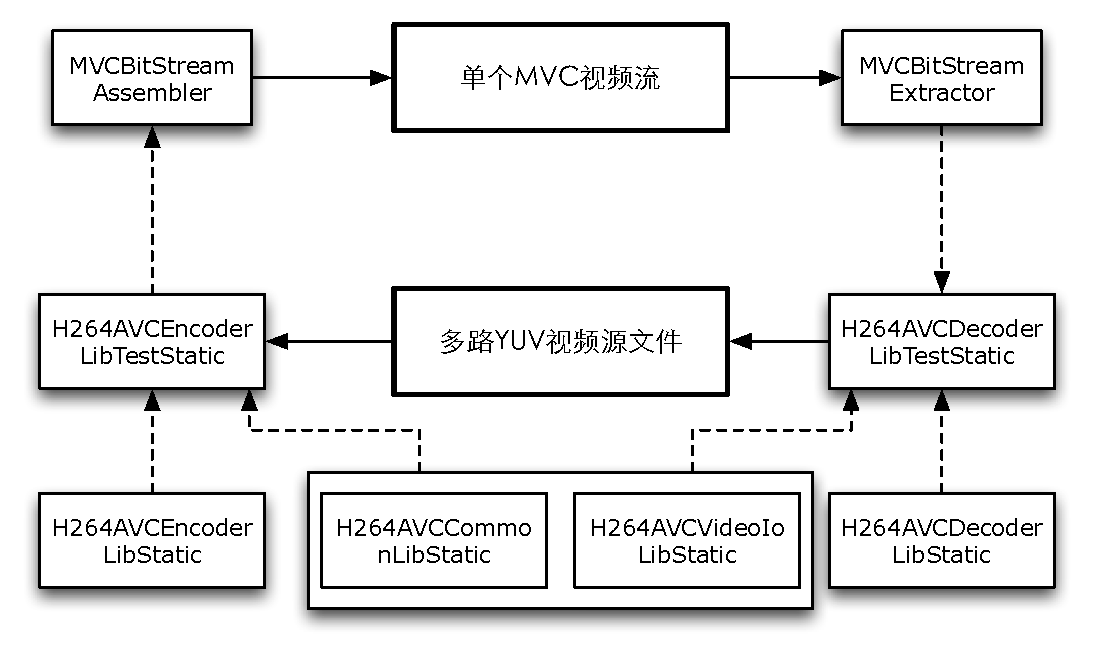
\includegraphics[width=0.8\textwidth]{JMVCstructure}
\caption{JMVC编解码框架}
\label{fig:JMVCstructure}
\end{center}
\end{figure}

利用JMVC进行编解码的框架如\autoref{fig:JMVCstructure}所示。

编码器的输入为若干路YUV视频,一般是同一场景从若干不同角度拍摄的视频,有相同的分辨率并且经过时间同步和校准。YUV文件要求是4:2:0格式,每$2\times2=4$个像素由一个$2\times2$的亮度矩阵和两个$1\times1$的色度矩阵。亮度矩阵顾名思义表示了4个像素的亮度,两个色度矩阵表示像素红蓝两色的平均色度,如\autoref{fig:Barn-yuv}所示。
在编解码器开发期间,庞一、胡伟栋、张凤研等对编解码在帧级别的并行性进行了深入研究\cite{pang2009adaptive,yi2008parallelized},并在编码器和解码器中都采用了帧并行的算法。

\begin{figure}[htbp]
\begin{center}
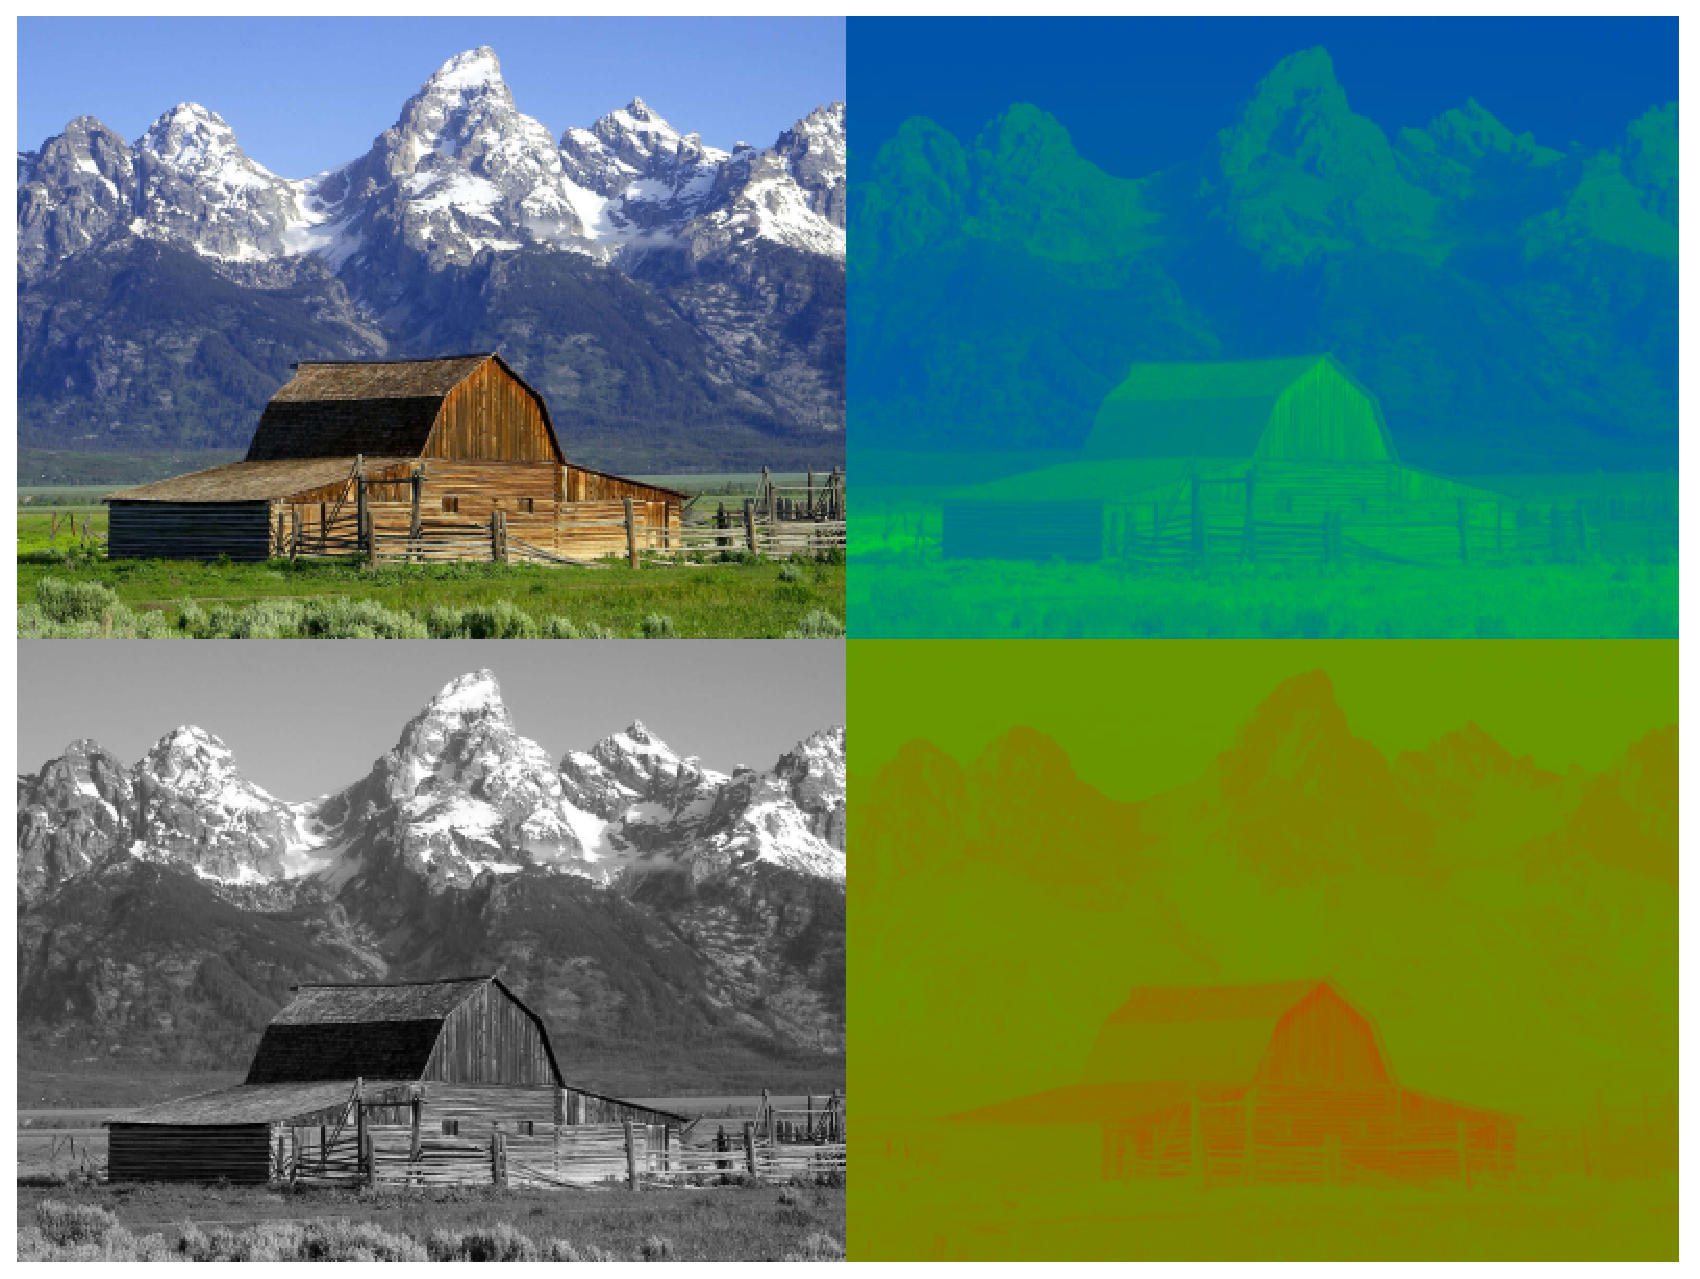
\includegraphics[scale=0.3]{Barn-yuv.eps}
\caption{原始图像(左上)和其Y'(左下)、U(右上)、V(右下)分量}
\label{fig:Barn-yuv}
\end{center}
\end{figure}

\section{自主开发的MVC解码器}
\label{sec:mvcdecoder}

我们根据参考软件和\onlinecite{richardson2003h}中的描述,实现了MVC的编解码器。其中,编码器的处理过程如\autoref{fig:mvcencoder}\footnote{《H.264 and MPEG-4 video compression, video coding for next-generation multimedia》\cite{richardson2003h}p.160}所示。解码器简单说来就是编码器的逆过程,其流程如\autoref{fig:mvcdecoder}\footnote{《H.264 and MPEG-4 video compression, video coding for next-generation multimedia》\cite{richardson2003h}p.161}所示。

%TODO 解码流程图
\begin{figure}[htbp]
\begin{center}
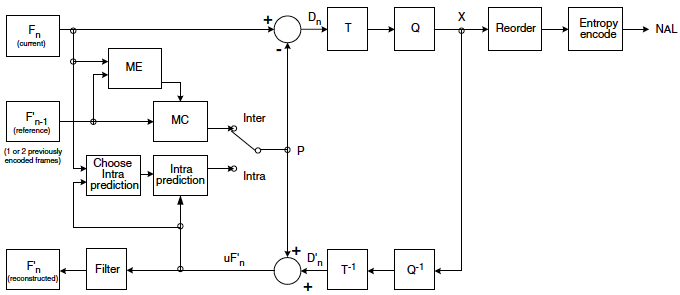
\includegraphics[width=\textwidth]{mvcencoder.png}
\caption{MVC Encoder流程图}
\label{fig:mvcencoder}
\end{center}
\end{figure}

\begin{figure}[htbp]
\begin{center}
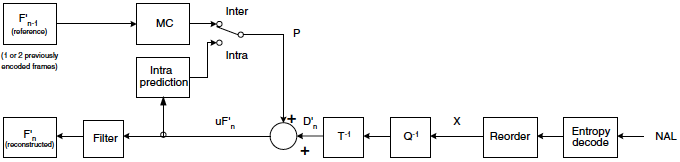
\includegraphics[width=\textwidth]{mvcdecoder.png}
\caption{MVC Decoder流程图}
\label{fig:mvcdecoder}
\end{center}
\end{figure}
%TODO 解码器行为描述
解码器中,在解码一帧之前,需要获得解码该帧所需要的全部参考帧,之后才能进行解码。所以说,帧的解码顺序与输入顺序是不一致的。在我们的解码器中,通过一个根据\onlinecite{pang2009framework}实现的调度器来安排解码顺序。我们的解码器有一个线程进行解码源数据的读取,在实验中,是读文件流;相应的,有一个线程进行解码输出的写操作,在实验中是写文件流;此外,调度器会根据参数配置,同时启用1个到N个线程执行解码任务,N不会大于设定的最大线程数。

\section{小结}
\label{sec:sum2}
本章主要介绍了参考软件JMVC的模块划分、功能以及我们自主开发的MVC解码器的基本结构和解码流程。

\cleardoublepage